\scanpage{69}
% archive foliation: 68
% lines 1--10
\begin{center}U N I V E R S I T E\\DES SCIENCES ET TECHNIQUES\\DU LANGUEDOC\\------------\\Service de la Scolarité\\MR/GJ\\Diffusion : Liste A\\N°:4000\end{center}
\begin{flushright}Montpellier, le 26 Juin 1978\end{flushright}
\begin{center}\uline{AVIS DE SOUTENANCE D'UNE THESE DE DOCTORAT D'UNIVERSITE}\end{center}
% lines 11--20
\uline{Nom et prénom du candidat} : PAYEN Jean-Luc

\uline{Titre de la thèse} : Contribution à l'étude de la protection des surfaces métalliques par les composés oxyfluorés du phosphore V.

\uline{Date, heure et lieu de soutenance prévus} :
\begin{quote}13 JUILLET 1978 à 11 Heures\\Ecole Nationale Supérieure de Chimie.\end{quote}
\uline{Nom du Directeur de thèse} :
\begin{quote}Monsieur le Professeur L. COT.\end{quote}
\uline{Désignation du laboratoire où la thèse est préparée} :
Laboratoire de Chimie minérale appliquée - Chimie des Matériaux, E. N. S. C. M.
% lines 21--28
\uline{Analyse de l'ouvrage} :

Les sels de l'anion $\mathrm{PO3F}^{2-}$ peuvent être utilisés lors de l'opération de post-traitement après phosphatation en substitution des sels de chrome VI hautement toxiques.

Une étude de la nature de la surface crée par phosphatation et passivation par K2PO3F a été entreprise par différentes techniques : ESCA,Microscopies électronique , et ionique. Elle montre une réorganisation physico chimique de la couche.
% lines 29--40
\uline{Durée approximative des recherches ayant abouti à la thèse} : 2 ans

\uline{Composition du jury proposé} :
\begin{quote}MM. :\\M. MAURIN\\L. COT\\P. DESRE\\J. DURAND\\X. GRANDIN DE L'EPREVIER\\B. PARANT\\P.R PHILIP\end{quote}
\begin{flushright}Le Secrétaire Général,\end{flushright}
\figure{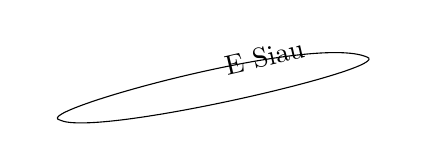
\begin{tikzpicture}[x=1cm,y=1cm]
\node[rotate=13] at (2.6,.55) {\unsure{E Siau}};
\draw (3.9,.55) .. controls (3.2,.85) and (-.4,-.15) .. (0,-.25) .. controls (.45,-.48) and (4.3,.42) .. (3.9,.55);
\end{tikzpicture}}
\begin{flushright}\uline{E. SIAU}\end{flushright}
